% =============================================================
% NutriTrack — Certification Defense Slides
% RNCP37638 — Expert in Massive Data Infrastructures
% Beamer presentation with Metropolis theme
% =============================================================
\documentclass[aspectratio=169, 10pt]{beamer}

% ── Theme ──────────────────────────────────────────────────────
\usetheme{metropolis}
\metroset{
  progressbar=frametitle,
  numbering=fraction,
  block=fill,
  sectionpage=progressbar
}

% ── Colors (NutriTrack green theme) ───────────────────────────
\definecolor{ntgreen}{HTML}{2E7D32}
\definecolor{ntlightgreen}{HTML}{66BB6A}
\definecolor{ntdarkgreen}{HTML}{1B5E20}
\definecolor{ntbg}{HTML}{FAFAFA}
\definecolor{ntaccent}{HTML}{FF8F00}
\definecolor{ntblue}{HTML}{1565C0}
\definecolor{ntred}{HTML}{C62828}
\definecolor{ntpurple}{HTML}{6A1B9A}
\definecolor{bronze}{HTML}{CD7F32}
\definecolor{silver}{HTML}{A0A0A0}
\definecolor{gold}{HTML}{DAA520}
\definecolor{demobox}{HTML}{FFF3E0}

\setbeamercolor{palette primary}{bg=ntgreen, fg=white}
\setbeamercolor{frametitle}{bg=ntgreen, fg=white}
\setbeamercolor{progress bar}{fg=ntaccent, bg=ntgreen!20}
\setbeamercolor{title separator}{fg=ntaccent}
\setbeamercolor{alerted text}{fg=ntaccent}
\setbeamercolor{example text}{fg=ntgreen}
\setbeamercolor{block title}{bg=ntgreen, fg=white}
\setbeamercolor{block body}{bg=ntgreen!5}
\setbeamercolor{block title alerted}{bg=ntred, fg=white}
\setbeamercolor{block body alerted}{bg=ntred!5}

% ── Packages ──────────────────────────────────────────────────
\usepackage[english]{babel}
\usepackage{tikz}
\usetikzlibrary{arrows.meta, positioning, shapes.geometric, calc, fit, decorations.pathreplacing}
\usepackage{fontawesome5}
\usepackage{booktabs}
\usepackage{graphicx}
\usepackage{listings}
\usepackage{multicol}
\usepackage{xcolor}
\usepackage{hyperref}

% ── Code listings ─────────────────────────────────────────────
\lstset{
  basicstyle=\tiny\ttfamily,
  breaklines=true,
  frame=single,
  backgroundcolor=\color{ntbg},
  keywordstyle=\color{ntblue}\bfseries,
  commentstyle=\color{gray},
  stringstyle=\color{ntgreen},
}

% ── Custom commands ───────────────────────────────────────────
\newcommand{\nutritrack}{\textsc{NutriTrack}}
\newcommand{\competency}[1]{\textbf{\color{ntblue}#1}}
\newcommand{\fullcov}{\textcolor{ntgreen}{\faCheckCircle}}
\newcommand{\partcov}{\textcolor{ntaccent}{\faExclamationTriangle}}

% Demo callout box
\newcommand{\democallout}[1]{%
  \begin{center}
  \begin{tikzpicture}
    \node[fill=demobox, rounded corners=8pt, inner sep=10pt,
          draw=ntaccent, line width=1.5pt] {%
      \Large\faDesktop\quad\textbf{\color{ntaccent}LIVE DEMO:} #1
    };
  \end{tikzpicture}
  \end{center}
}

% ── Title ─────────────────────────────────────────────────────
\title{\nutritrack}
\subtitle{Nutritional Data Engineering Platform}
\author{Reetika Gautam}
\date{March 2026}
\institute{%
  RNCP37638 --- Expert in Massive Data Infrastructures\\
  Level 7 (Master's equivalent) \quad\textbullet\quad Simplon.co
}

% =============================================================
\begin{document}

% ─────────────────────────────────────────────────────────────
% TITLE SLIDE
% ─────────────────────────────────────────────────────────────
\begin{frame}[standout]
  \begin{tikzpicture}[remember picture, overlay]
    \node[circle, fill=white, minimum size=1.8cm, text=ntgreen,
          font=\Huge\bfseries] at ([yshift=2.5cm]current page.center) {NT};
  \end{tikzpicture}
  \vspace{1.5cm}

  {\Huge\bfseries \nutritrack}\\[0.3cm]
  {\large Nutritional Data Engineering Platform}\\[0.8cm]
  {\normalsize Reetika Gautam}\\[0.2cm]
  {\small RNCP37638 --- Expert in Massive Data Infrastructures}\\
  {\small Level 7 $\bullet$ March 2026 $\bullet$ Simplon.co}
\end{frame}

% ─────────────────────────────────────────────────────────────
% AGENDA
% ─────────────────────────────────────────────────────────────
\begin{frame}{Defense Agenda}
\begin{columns}[T]
\begin{column}{0.55\textwidth}
  \begin{enumerate}
    \item[\faProjectDiagram] \textbf{E1--E5} --- Project \& Implementation \hfill \textit{60 min}
    \begin{itemize}
      \item E1: Need Analysis (C1)
      \item E2: Architecture \& Monitoring (C1--C4, C6)
      \item E3: Project Kickoff Simulation (C5--C7)
      \item E4: Data Collection \& API (C8--C12)
      \item E5: Data Warehouse (C13--C15)
    \end{itemize}
    \item[\faComments] \textbf{E6} --- DW Maintenance Q\&A \hfill \textit{10 min}
    \item[\faCloud] \textbf{E7} --- Data Lake \hfill \textit{10 min}
    \item[\faQuestion] \textbf{Jury Questions} \hfill \textit{10 min}
  \end{enumerate}
\end{column}
\begin{column}{0.4\textwidth}
  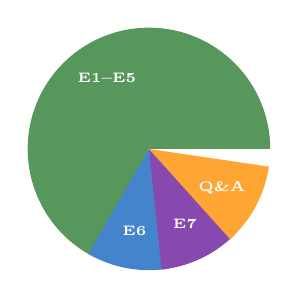
\begin{tikzpicture}[scale=0.7]
    \foreach \angle/\label/\col/\pct in {
      0/E1--E5/ntgreen/67,
      240/E6/ntblue/11,
      276/E7/ntpurple/11,
      312/Q\&A/ntaccent/11
    } {
      \fill[\col!80] (0,0) -- (\angle:2.2) arc (\angle:\angle+\pct*3.6:2.2) -- cycle;
      \node[font=\tiny\bfseries, white] at (\angle+\pct*1.8:1.5) {\label};
    }
  \end{tikzpicture}
\end{column}
\end{columns}

\note{
  Welcome the jury. Explain the 90-minute structure.
  Mention live demos throughout the presentation.
  E1--E5 is the main body, E6 is Q\&A-based, E7 covers data lake.
}
\end{frame}

% ─────────────────────────────────────────────────────────────
% PROJECT OVERVIEW (2 slides)
% ─────────────────────────────────────────────────────────────
\begin{frame}{Project Context}
\begin{columns}[T]
\begin{column}{0.55\textwidth}
  \textbf{Problem:} Nutritional data is scattered, inconsistent,\\
  and hard to analyze at scale.\\[0.5cm]

  \textbf{Solution:} \nutritrack{} --- an end-to-end data engineering\\
  platform for nutritional data analysis.\\[0.5cm]

  \textbf{Key numbers:}
  \begin{itemize}
    \item 3M+ products from Open Food Facts
    \item 15 Docker services
    \item 7 Airflow DAGs
    \item 56 automated tests
    \item 6 Grafana dashboards
  \end{itemize}
\end{column}
\begin{column}{0.4\textwidth}
  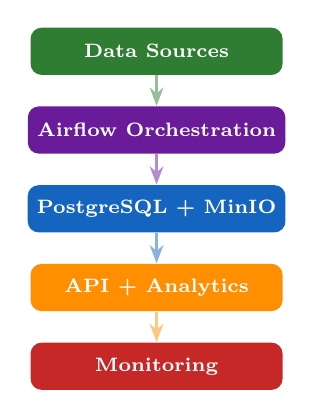
\begin{tikzpicture}[
    every node/.style={font=\scriptsize, align=center},
    layer/.style={rounded corners=4pt, minimum width=3.2cm,
                  minimum height=0.6cm, text=white, font=\scriptsize\bfseries}
  ]
    \node[layer, fill=ntgreen] (src) at (0,4) {Data Sources};
    \node[layer, fill=ntpurple] (orch) at (0,3) {Airflow Orchestration};
    \node[layer, fill=ntblue] (store) at (0,2) {PostgreSQL + MinIO};
    \node[layer, fill=ntaccent] (app) at (0,1) {API + Analytics};
    \node[layer, fill=ntred] (mon) at (0,0) {Monitoring};

    \draw[-{Stealth}, thick, ntgreen!50] (src) -- (orch);
    \draw[-{Stealth}, thick, ntpurple!50] (orch) -- (store);
    \draw[-{Stealth}, thick, ntblue!50] (store) -- (app);
    \draw[-{Stealth}, thick, ntaccent!50] (app) -- (mon);
  \end{tikzpicture}
\end{column}
\end{columns}

\note{
  Set the context. NutriTrack solves data fragmentation in nutrition.
  Emphasize scale: 3M products, 15 services, full CI/CD.
}
\end{frame}

\begin{frame}{Tech Stack}
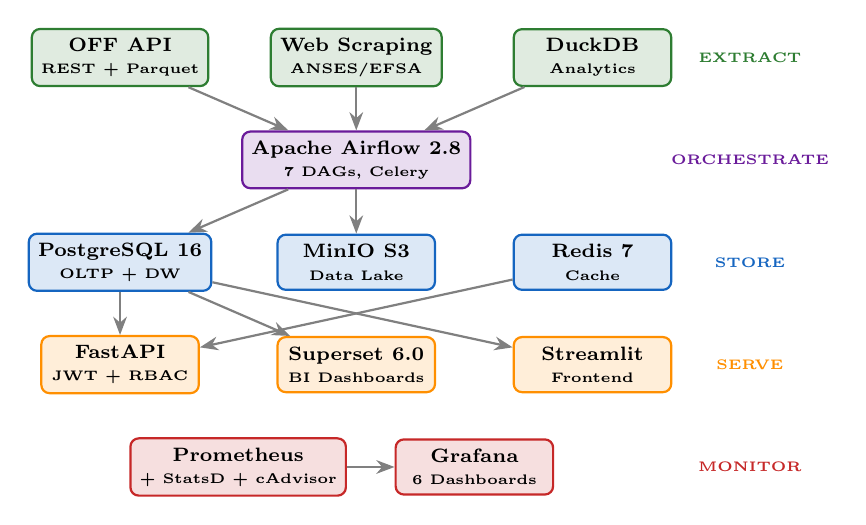
\begin{tikzpicture}[
  every node/.style={font=\scriptsize, align=center},
  box/.style={rounded corners=3pt, minimum width=2cm, minimum height=0.7cm,
              draw, thick, font=\scriptsize\bfseries},
]
  % Row 1 - Sources
  \node[box, fill=ntgreen!15, draw=ntgreen] (off) at (0,0) {OFF API\\{\tiny REST + Parquet}};
  \node[box, fill=ntgreen!15, draw=ntgreen] (scr) at (3,0) {Web Scraping\\{\tiny ANSES/EFSA}};
  \node[box, fill=ntgreen!15, draw=ntgreen] (db) at (6,0) {DuckDB\\{\tiny Analytics}};

  % Row 2 - Orchestration
  \node[box, fill=ntpurple!15, draw=ntpurple] (af) at (3,-1.3) {Apache Airflow 2.8\\{\tiny 7 DAGs, Celery}};

  % Row 3 - Storage
  \node[box, fill=ntblue!15, draw=ntblue] (pg) at (0,-2.6) {PostgreSQL 16\\{\tiny OLTP + DW}};
  \node[box, fill=ntblue!15, draw=ntblue] (mn) at (3,-2.6) {MinIO S3\\{\tiny Data Lake}};
  \node[box, fill=ntblue!15, draw=ntblue] (rd) at (6,-2.6) {Redis 7\\{\tiny Cache}};

  % Row 4 - Apps
  \node[box, fill=ntaccent!15, draw=ntaccent] (api) at (0,-3.9) {FastAPI\\{\tiny JWT + RBAC}};
  \node[box, fill=ntaccent!15, draw=ntaccent] (ss) at (3,-3.9) {Superset 6.0\\{\tiny BI Dashboards}};
  \node[box, fill=ntaccent!15, draw=ntaccent] (st) at (6,-3.9) {Streamlit\\{\tiny Frontend}};

  % Row 5 - Monitoring
  \node[box, fill=ntred!15, draw=ntred] (pr) at (1.5,-5.2) {Prometheus\\{\tiny + StatsD + cAdvisor}};
  \node[box, fill=ntred!15, draw=ntred] (gf) at (4.5,-5.2) {Grafana\\{\tiny 6 Dashboards}};

  % Arrows
  \draw[-{Stealth}, thick, gray] (off) -- (af);
  \draw[-{Stealth}, thick, gray] (scr) -- (af);
  \draw[-{Stealth}, thick, gray] (db) -- (af);
  \draw[-{Stealth}, thick, gray] (af) -- (pg);
  \draw[-{Stealth}, thick, gray] (af) -- (mn);
  \draw[-{Stealth}, thick, gray] (pg) -- (api);
  \draw[-{Stealth}, thick, gray] (pg) -- (ss);
  \draw[-{Stealth}, thick, gray] (rd) -- (api);
  \draw[-{Stealth}, thick, gray] (pg) -- (st);
  \draw[-{Stealth}, thick, gray] (pr) -- (gf);

  % Labels
  \node[font=\tiny\bfseries, ntgreen] at (8,0) {EXTRACT};
  \node[font=\tiny\bfseries, ntpurple] at (8,-1.3) {ORCHESTRATE};
  \node[font=\tiny\bfseries, ntblue] at (8,-2.6) {STORE};
  \node[font=\tiny\bfseries, ntaccent] at (8,-3.9) {SERVE};
  \node[font=\tiny\bfseries, ntred] at (8,-5.2) {MONITOR};
\end{tikzpicture}

\note{
  Walk through the stack layer by layer.
  Emphasize all open-source, containerized with Docker Compose.
  15 services, single-command deployment.
}
\end{frame}

% =============================================================
\section{E1 --- Need Analysis (C1)}
% =============================================================

\begin{frame}{Interview Grids \competency{C1}}
\begin{columns}[T]
\begin{column}{0.48\textwidth}
  \textbf{\faUsers\ Data Producers}
  \begin{enumerate}\small
    \item Business activities involved
    \item Data types generated
    \item Data formats \& volumes
    \item Update frequency
    \item Quality controls
    \item Metadata available
    \item Access conditions
    \item Storage constraints
    \item Applied treatments
    \item Known issues
  \end{enumerate}
\end{column}
\begin{column}{0.48\textwidth}
  \textbf{\faChartBar\ Data Consumers}
  \begin{enumerate}\small
    \item Analysis objectives
    \item Required granularity
    \item Delivery format needs
    \item Update frequency needs
    \item Current data gaps
    \item Quality expectations
    \item Tool preferences
    \item Access requirements
    \item RGPD constraints
    \item Accessibility needs
  \end{enumerate}
\end{column}
\end{columns}

\note{
  Explain both grids. Producers = OFF API, ANSES.
  Consumers = nutritionists, end-users, data scientists.
  Grids question business activities AND data characterization.
}
\end{frame}

\begin{frame}{Synthesis Note \competency{C1}}
\begin{block}{SMART Objectives}
  \begin{itemize}
    \item \textbf{S}pecific: Centralize nutritional data from 5+ sources
    \item \textbf{M}easurable: 50,000+ products, <5s query response
    \item \textbf{A}chievable: Open-source stack, Docker-based
    \item \textbf{R}elevant: Address fragmented nutrition data landscape
    \item \textbf{T}ime-bound: 12-week implementation timeline
  \end{itemize}
\end{block}

\vspace{0.3cm}
\textbf{Pre-project includes:}
\begin{itemize}
  \item Macro technical recommendations
  \item RGPD compliance actions identified
  \item Accessibility accommodations planned
  \item RICE analysis for feature prioritization
\end{itemize}

\note{
  Key deliverable for C1. Show how objectives drive architecture.
  RICE = Reach, Impact, Confidence, Effort.
}
\end{frame}

% =============================================================
\section{E2 --- Architecture \& Technical Study (C2, C3, C4, C6)}
% =============================================================

\begin{frame}{Data Topography \competency{C2}}
\small
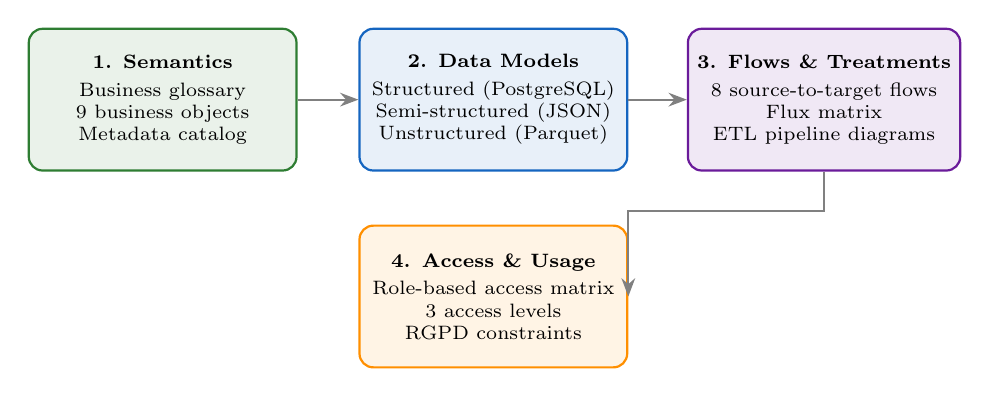
\begin{tikzpicture}[
  part/.style={rounded corners=5pt, minimum width=3.4cm, minimum height=1.8cm,
               draw, thick, align=center, font=\scriptsize},
]
  \node[part, fill=ntgreen!10, draw=ntgreen] (sem) at (0,0) {
    \textbf{1. Semantics}\\[2pt]
    Business glossary\\
    9 business objects\\
    Metadata catalog
  };
  \node[part, fill=ntblue!10, draw=ntblue] (mod) at (4.2,0) {
    \textbf{2. Data Models}\\[2pt]
    Structured (PostgreSQL)\\
    Semi-structured (JSON)\\
    Unstructured (Parquet)
  };
  \node[part, fill=ntpurple!10, draw=ntpurple] (flow) at (8.4,0) {
    \textbf{3. Flows \& Treatments}\\[2pt]
    8 source-to-target flows\\
    Flux matrix\\
    ETL pipeline diagrams
  };
  \node[part, fill=ntaccent!10, draw=ntaccent] (acc) at (4.2,-2.5) {
    \textbf{4. Access \& Usage}\\[2pt]
    Role-based access matrix\\
    3 access levels\\
    RGPD constraints
  };

  \draw[-{Stealth}, thick, gray] (sem) -- (mod);
  \draw[-{Stealth}, thick, gray] (mod) -- (flow);
  \draw[-{Stealth}, thick, gray] (flow.south) -- ++(0,-0.5) -| (acc.east);
\end{tikzpicture}

\note{
  C2 requires 4-part topography. Walk through each quadrant.
  The flux matrix shows all 8 data flows with formats and frequencies.
}
\end{frame}

\begin{frame}{System Architecture \competency{C3}}
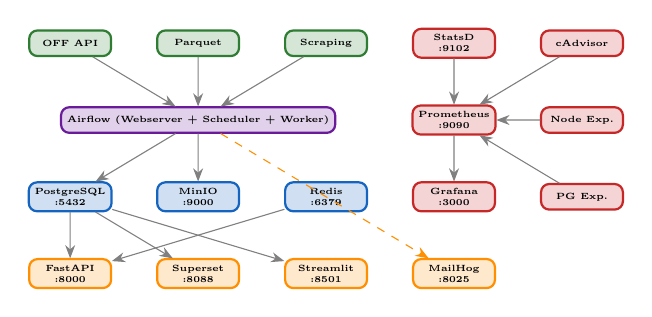
\begin{tikzpicture}[scale=0.65, transform shape,
  svc/.style={rounded corners=3pt, minimum width=1.6cm, minimum height=0.5cm,
              draw, thick, font=\tiny\bfseries, align=center}
]
  % Sources
  \node[svc, fill=ntgreen!20, draw=ntgreen] (s1) at (0,5) {OFF API};
  \node[svc, fill=ntgreen!20, draw=ntgreen] (s2) at (2.5,5) {Parquet};
  \node[svc, fill=ntgreen!20, draw=ntgreen] (s3) at (5,5) {Scraping};

  % Airflow
  \node[svc, fill=ntpurple!20, draw=ntpurple, minimum width=5cm] (af) at (2.5,3.5) {Airflow (Webserver + Scheduler + Worker)};

  % Storage
  \node[svc, fill=ntblue!20, draw=ntblue] (pg) at (0,2) {PostgreSQL\\:5432};
  \node[svc, fill=ntblue!20, draw=ntblue] (mn) at (2.5,2) {MinIO\\:9000};
  \node[svc, fill=ntblue!20, draw=ntblue] (rd) at (5,2) {Redis\\:6379};

  % Apps
  \node[svc, fill=ntaccent!20, draw=ntaccent] (api) at (0,0.5) {FastAPI\\:8000};
  \node[svc, fill=ntaccent!20, draw=ntaccent] (ss) at (2.5,0.5) {Superset\\:8088};
  \node[svc, fill=ntaccent!20, draw=ntaccent] (st) at (5,0.5) {Streamlit\\:8501};

  % Monitoring
  \node[svc, fill=ntred!20, draw=ntred] (pr) at (7.5,3.5) {Prometheus\\:9090};
  \node[svc, fill=ntred!20, draw=ntred] (gf) at (7.5,2) {Grafana\\:3000};
  \node[svc, fill=ntred!20, draw=ntred] (sd) at (7.5,5) {StatsD\\:9102};
  \node[svc, fill=ntred!20, draw=ntred] (ca) at (10,5) {cAdvisor};
  \node[svc, fill=ntred!20, draw=ntred] (ne) at (10,3.5) {Node Exp.};
  \node[svc, fill=ntred!20, draw=ntred] (pe) at (10,2) {PG Exp.};
  \node[svc, fill=ntaccent!20, draw=ntaccent] (mh) at (7.5,0.5) {MailHog\\:8025};

  % Arrows
  \foreach \s in {s1,s2,s3} \draw[-{Stealth}, gray] (\s) -- (af);
  \draw[-{Stealth}, gray] (af) -- (pg);
  \draw[-{Stealth}, gray] (af) -- (mn);
  \draw[-{Stealth}, gray] (pg) -- (api);
  \draw[-{Stealth}, gray] (pg) -- (ss);
  \draw[-{Stealth}, gray] (pg) -- (st);
  \draw[-{Stealth}, gray] (rd) -- (api);
  \draw[-{Stealth}, gray] (sd) -- (pr);
  \draw[-{Stealth}, gray] (ca) -- (pr);
  \draw[-{Stealth}, gray] (ne) -- (pr);
  \draw[-{Stealth}, gray] (pe) -- (pr);
  \draw[-{Stealth}, gray] (pr) -- (gf);
  \draw[-{Stealth}, dashed, ntaccent] (af) -- (mh);
\end{tikzpicture}

\note{
  15 Docker services. All containerized, single docker compose up.
  Highlight the 5 layers: sources, orchestration, storage, apps, monitoring.
}
\end{frame}

\begin{frame}{Technical Monitoring \competency{C4}}
\begin{block}{Technology Watch Newsletter}
  \begin{itemize}
    \item \textbf{Apache Superset 6.0} --- Migration from 4.x, new viz types
    \item \textbf{GDPR Update} --- EDPB Guidelines 01/2026
    \item \textbf{Apache Airflow 2.8} --- New features, performance improvements
  \end{itemize}
\end{block}

\vspace{0.3cm}
\begin{columns}[T]
\begin{column}{0.48\textwidth}
  \textbf{Source reliability criteria:}
  \begin{itemize}\small
    \item Official documentation
    \item Peer-reviewed guidelines
    \item Community-maintained APIs
    \item Regulatory publications
  \end{itemize}
\end{column}
\begin{column}{0.48\textwidth}
  \textbf{Monitoring schedule:}
  \begin{itemize}\small
    \item Minimum 1 hour/week
    \item Published via MkDocs site
    \item Accessible to all stakeholders
    \item Action items tracked
  \end{itemize}
\end{column}
\end{columns}

\note{
  C4 requires a veille technologique. Show the newsletter.
  Emphasize source reliability criteria and regular schedule.
}
\end{frame}

% =============================================================
\section{E3 --- Project Kickoff (C5, C6, C7)}
% =============================================================

\begin{frame}{Project Planning \competency{C5}}
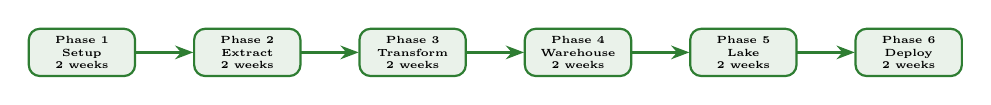
\begin{tikzpicture}[scale=0.75, transform shape,
  phase/.style={rounded corners=4pt, minimum width=1.8cm, minimum height=0.8cm,
                draw=ntgreen, thick, fill=ntgreen!10, font=\tiny\bfseries, align=center}
]
  \node[phase] (p1) at (0,0) {Phase 1\\Setup\\{\tiny 2 weeks}};
  \node[phase] (p2) at (2.8,0) {Phase 2\\Extract\\{\tiny 2 weeks}};
  \node[phase] (p3) at (5.6,0) {Phase 3\\Transform\\{\tiny 2 weeks}};
  \node[phase] (p4) at (8.4,0) {Phase 4\\Warehouse\\{\tiny 2 weeks}};
  \node[phase] (p5) at (11.2,0) {Phase 5\\Lake\\{\tiny 2 weeks}};
  \node[phase] (p6) at (14,0) {Phase 6\\Deploy\\{\tiny 2 weeks}};

  \draw[-{Stealth}, thick, ntgreen] (p1) -- (p2);
  \draw[-{Stealth}, thick, ntgreen] (p2) -- (p3);
  \draw[-{Stealth}, thick, ntgreen] (p3) -- (p4);
  \draw[-{Stealth}, thick, ntgreen] (p4) -- (p5);
  \draw[-{Stealth}, thick, ntgreen] (p5) -- (p6);
\end{tikzpicture}

\vspace{0.5cm}
\begin{columns}[T]
\begin{column}{0.48\textwidth}
  \textbf{Effort Weighting:} Fibonacci story points\\[0.2cm]
  \textbf{Rituals:}
  \begin{itemize}\small
    \item Sprint planning (bi-weekly)
    \item Daily standup
    \item Sprint review \& demo
    \item Retrospective
  \end{itemize}
\end{column}
\begin{column}{0.48\textwidth}
  \textbf{Team Composition:}
  \begin{itemize}\small
    \item Data Engineer (lead)
    \item Platform Engineer
    \item CI/CD Engineer
    \item Certification Auditor
    \item Technical Reviewer
  \end{itemize}
\end{column}
\end{columns}

\note{
  C5: Show the 6-phase roadmap. Fibonacci points for estimation.
  Calendar with tasks, deliverables, resource attribution.
}
\end{frame}

\begin{frame}{Supervision \& Communication \competency{C6} \competency{C7}}
\begin{columns}[T]
\begin{column}{0.48\textwidth}
  \textbf{C6 --- Tracking Indicators:}
  \begin{itemize}\small
    \item Airflow DAG success/failure rates
    \item \texttt{etl\_activity\_log} table\\(22 entries spanning 14 days)
    \item Records extracted/loaded/rejected
    \item Data completeness percentage
    \item ETL duration trends
  \end{itemize}
  \vspace{0.3cm}
  \textbf{Tracking tools:}
  \begin{itemize}\small
    \item Airflow UI
    \item Grafana SLA dashboard
    \item Git version control
  \end{itemize}
\end{column}
\begin{column}{0.48\textwidth}
  \textbf{C7 --- Communication Strategy:}
  \begin{itemize}\small
    \item Sprint kickoff presentations
    \item Progress update reports
    \item Technical demos (live)
    \item API docs (Swagger/ReDoc)
    \item User docs (MkDocs site)
    \item Final delivery (this defense)
  \end{itemize}
  \vspace{0.3cm}
  \textbf{Audience adaptation:}
  \begin{itemize}\small
    \item Technical: Swagger, Grafana
    \item Business: Streamlit, Superset
    \item Jury: Report + slides + demo
  \end{itemize}
\end{column}
\end{columns}

\note{
  C6: Show the populated activity log. Indicators updated throughout.
  C7: Multi-audience communication. MkDocs for browsable docs.
}
\end{frame}

% =============================================================
\section{E4 --- Data Collection \& API (C8--C12)}
% =============================================================

\begin{frame}{5 Extraction Sources \competency{C8}}
\begin{tikzpicture}[
  src/.style={rounded corners=4pt, minimum width=2.6cm, minimum height=1cm,
              draw, thick, font=\scriptsize, align=center}
]
  \node[src, fill=ntgreen!15, draw=ntgreen] (a) at (0,0) {\faGlobe\ REST API\\{\tiny extract\_off\_api.py}\\{\tiny Daily, 1000+ products}};
  \node[src, fill=ntblue!15, draw=ntblue] (b) at (4,0) {\faDatabase\ Data File\\{\tiny extract\_off\_parquet.py}\\{\tiny Weekly, 50k products}};
  \node[src, fill=ntpurple!15, draw=ntpurple] (c) at (8,0) {\faCode\ Web Scraping\\{\tiny extract\_scraping.py}\\{\tiny Monthly, guidelines}};
  \node[src, fill=ntaccent!15, draw=ntaccent] (d) at (2,-2) {\faServer\ Database\\{\tiny extract\_from\_db.py}\\{\tiny On-demand}};
  \node[src, fill=ntred!15, draw=ntred] (e) at (6,-2) {\faCubes\ Big Data\\{\tiny extract\_duckdb.py}\\{\tiny DuckDB analytics}};

  \node[rounded corners=6pt, fill=ntgreen!5, draw=ntgreen, thick,
        minimum width=3cm, minimum height=0.8cm, font=\scriptsize\bfseries]
        (out) at (4,-4) {aggregate\_clean.py};

  \draw[-{Stealth}, thick, gray] (a.south) -- ++(0,-0.3) -| (out.north);
  \draw[-{Stealth}, thick, gray] (b) -- (out);
  \draw[-{Stealth}, thick, gray] (c.south) -- ++(0,-0.3) -| (out.north);
  \draw[-{Stealth}, thick, gray] (d) -- (out);
  \draw[-{Stealth}, thick, gray] (e) -- (out);
\end{tikzpicture}

\note{
  C8 requires extraction from: REST API, data file, scraping, database, big data system.
  All 5 covered. Each script has: entry point, error handling, result saving, Git versioned.
}
\end{frame}

\begin{frame}{SQL Queries \& Data Aggregation \competency{C9} \competency{C10}}
\begin{columns}[T]
\begin{column}{0.48\textwidth}
  \textbf{C9 --- 7 Optimized SQL Queries:}
  \begin{enumerate}\small
    \item Full-text search (GIN index)
    \item User nutrition summary (window fn)
    \item Product market analysis (CTE)
    \item Brand comparison (analytical)
    \item Temporal trends (LAG)
    \item Aggregation with HAVING
    \item Complex joins (materialized)
  \end{enumerate}
  \vspace{0.2cm}
  {\small All include \texttt{EXPLAIN ANALYZE} notes.}
\end{column}
\begin{column}{0.48\textwidth}
  \textbf{C10 --- Cleaning Pipeline:}
  \begin{enumerate}\small
    \item Column standardization (30+ mappings)
    \item Barcode cleaning (8--14 digits)
    \item Null product name removal
    \item Range validation (physiological max)
    \item Nutri-Score normalization (A--E)
    \item Deduplication by barcode
    \item Quality report generation
  \end{enumerate}
  \vspace{0.2cm}
  {\small Output: \texttt{products\_cleaned.parquet}}
\end{column}
\end{columns}

\note{
  C9: Show the analytical queries file. Highlight optimization choices.
  C10: Walk through cleaning steps. Mention the quality report.
}
\end{frame}

\begin{frame}{Database \& REST API \competency{C11} \competency{C12}}
\begin{columns}[T]
\begin{column}{0.48\textwidth}
  \textbf{C11 --- RGPD-Compliant Database:}
  \begin{itemize}\small
    \item MERISE models (MCD/MLD/MPD)
    \item PostgreSQL 16 with 8 tables
    \item \texttt{rgpd\_data\_registry} table
    \item Consent tracking columns
    \item Automated \texttt{rgpd\_cleanup\_expired\_data()}
    \item Password hashing (bcrypt)
    \item UUID-based identification
  \end{itemize}
\end{column}
\begin{column}{0.48\textwidth}
  \textbf{C12 --- FastAPI REST API:}
  \begin{itemize}\small
    \item OpenAPI 3.0 (Swagger + ReDoc)
    \item JWT authentication (60-min expiry)
    \item Role-based access (user, nutritionist, admin)
    \item Endpoints: auth, products, meals
    \item Full-text search with pagination
    \item Redis-cached daily summaries
  \end{itemize}
\end{column}
\end{columns}

\vspace{0.3cm}
\democallout{Show Swagger UI at localhost:8000/docs}

\note{
  C11: Show the schema diagram. Emphasize RGPD compliance.
  C12: Open Swagger UI and demonstrate product search + auth flow.
}
\end{frame}

% =============================================================
\section{E5 --- Data Warehouse (C13--C15)}
% =============================================================

\begin{frame}{Star Schema \competency{C13}}
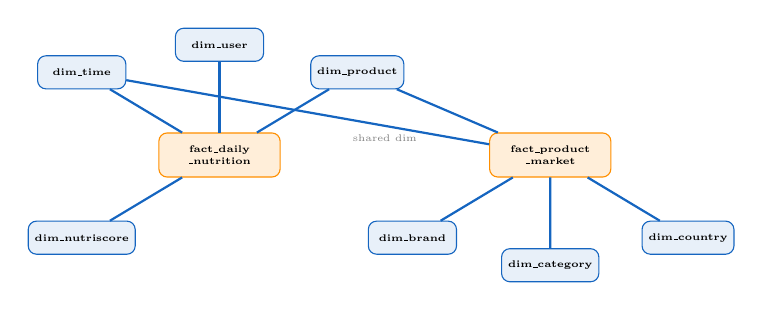
\begin{tikzpicture}[scale=0.7, transform shape,
  dim/.style={rounded corners=3pt, minimum width=1.6cm, minimum height=0.6cm,
              draw=ntblue, fill=ntblue!10, font=\tiny\bfseries, align=center},
  fact/.style={rounded corners=3pt, minimum width=2.2cm, minimum height=0.8cm,
               draw=ntaccent, fill=ntaccent!15, font=\tiny\bfseries, align=center}
]
  % Facts
  \node[fact] (f1) at (0,0) {fact\_daily\\\_nutrition};
  \node[fact] (f2) at (6,0) {fact\_product\\\_market};

  % Dimensions around f1
  \node[dim] (d1) at (-2.5,1.5) {dim\_time};
  \node[dim] (d2) at (0,2) {dim\_user};
  \node[dim] (d3) at (2.5,1.5) {dim\_product};
  \node[dim] (d7) at (-2.5,-1.5) {dim\_nutriscore};

  % Dimensions around f2
  \node[dim] (d4) at (3.5,-1.5) {dim\_brand};
  \node[dim] (d5) at (6,-2) {dim\_category};
  \node[dim] (d6) at (8.5,-1.5) {dim\_country};

  % Lines
  \draw[thick, ntblue] (d1) -- (f1);
  \draw[thick, ntblue] (d2) -- (f1);
  \draw[thick, ntblue] (d3) -- (f1);
  \draw[thick, ntblue] (d7) -- (f1);
  \draw[thick, ntblue] (d3) -- (f2);
  \draw[thick, ntblue] (d1) -- (f2);
  \draw[thick, ntblue] (d4) -- (f2);
  \draw[thick, ntblue] (d5) -- (f2);
  \draw[thick, ntblue] (d6) -- (f2);

  % Labels
  \node[font=\tiny, gray] at (3,0.3) {shared dim};
\end{tikzpicture}

\vspace{0.3cm}
\begin{columns}[T]
\begin{column}{0.48\textwidth}
  \textbf{7 Dimensions:} time, product, brand,\\category, country, user, nutriscore
\end{column}
\begin{column}{0.48\textwidth}
  \textbf{2 Facts:} daily nutrition (user meals),\\product market (supply tracking)
\end{column}
\end{columns}
\vspace{0.2cm}
{\small\textbf{Approach:} Bottom-up (Kimball) --- business requirements drove the schema.}

\note{
  C13: Star schema with shared dimensions. Bottom-up justified.
  7 dims, 2 facts, 6 datamart views.
}
\end{frame}

\begin{frame}{ETL Pipelines \& SCD \competency{C14} \competency{C15} \competency{C17}}
\begin{columns}[T]
\begin{column}{0.55\textwidth}
  \textbf{7 Airflow DAGs:}
  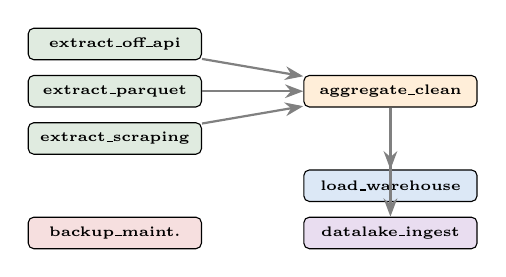
\begin{tikzpicture}[
    dag/.style={rounded corners=2pt, minimum width=2.2cm, minimum height=0.4cm,
                draw, font=\tiny\bfseries, align=center}
  ]
    \node[dag, fill=ntgreen!15] (e1) at (0,0) {extract\_off\_api};
    \node[dag, fill=ntgreen!15] (e2) at (0,-0.6) {extract\_parquet};
    \node[dag, fill=ntgreen!15] (e3) at (0,-1.2) {extract\_scraping};
    \node[dag, fill=ntaccent!15] (c) at (3.5,-0.6) {aggregate\_clean};
    \node[dag, fill=ntblue!15] (dw) at (3.5,-1.8) {load\_warehouse};
    \node[dag, fill=ntpurple!15] (dl) at (3.5,-2.4) {datalake\_ingest};
    \node[dag, fill=ntred!15] (bk) at (0,-2.4) {backup\_maint.};

    \draw[-{Stealth}, gray, thick] (e1) -- (c);
    \draw[-{Stealth}, gray, thick] (e2) -- (c);
    \draw[-{Stealth}, gray, thick] (e3) -- (c);
    \draw[-{Stealth}, gray, thick] (c) -- (dw);
    \draw[-{Stealth}, gray, thick] (c) -- (dl);
  \end{tikzpicture}
\end{column}
\begin{column}{0.42\textwidth}
  \textbf{SCD Implementation (C17):}\\[0.2cm]
  \begin{tabular}{ll}\small
    \textbf{Type 1} & dim\_brand\\
    & {\tiny Overwrite corrections}\\[0.15cm]
    \textbf{Type 2} & dim\_product\\
    & {\tiny Full history tracking}\\[0.15cm]
    \textbf{Type 3} & dim\_country\\
    & {\tiny Previous value column}\\
  \end{tabular}
  \vspace{0.3cm}

  {\small Change detection via\\\texttt{IS DISTINCT FROM}}
\end{column}
\end{columns}

\vspace{0.3cm}
\democallout{Show Airflow UI at localhost:8080}

\note{
  C14: DW is functional, Docker-based, Superset connected.
  C15: ETL loads dimensions then facts. ExternalTaskSensor for cross-DAG deps.
  C17: All 3 SCD types implemented and integrated into ETL.
}
\end{frame}

% =============================================================
\section{E6 --- DW Maintenance (C16, C17)}
% =============================================================

\begin{frame}{Alerting \& SLA Dashboard \competency{C16}}
\begin{columns}[T]
\begin{column}{0.48\textwidth}
  \textbf{Alert System:}
  \begin{itemize}\small
    \item \texttt{alerting.py} plugin --- callbacks for failure, retry, SLA miss, success
    \item Structured logging to \texttt{etl\_activity\_log}
    \item Email via MailHog SMTP
    \item StatsD metrics $\to$ Prometheus $\to$ Grafana
  \end{itemize}
  \vspace{0.2cm}
  \textbf{ITIL Priority Matrix:}\\[0.1cm]
  {\scriptsize
  \begin{tabular}{lll}
    \toprule
    \textbf{P1} & Critical & $<$1h response\\
    \textbf{P2} & High & $<$4h response\\
    \textbf{P3} & Medium & $<$24h response\\
    \textbf{P4} & Low & Next sprint\\
    \bottomrule
  \end{tabular}}
\end{column}
\begin{column}{0.48\textwidth}
  \textbf{SLA Dashboard (10 panels):}
  \begin{itemize}\small
    \item ETL success rate ($>$95\%)
    \item Data freshness ($<$24h)
    \item Backup completion (100\%)
    \item Query response time ($<$5s)
    \item 7-day success trend
    \item DAG run outcomes
    \item Storage usage
    \item SLA compliance table
  \end{itemize}
  \vspace{0.2cm}
  \textbf{Escalation:} L1 $\to$ L2 $\to$ L3
\end{column}
\end{columns}

\vspace{0.2cm}
\democallout{Show Grafana SLA dashboard + MailHog alerts}

\note{
  C16: This is the E6 Q\&A section. Be ready for deep questions.
  Show the SLA dashboard. Trigger a failure to show alert flow.
  Backup procedures: full + partial to MinIO.
}
\end{frame}

% =============================================================
\section{E7 --- Data Lake (C18--C21)}
% =============================================================

\begin{frame}{Medallion Architecture \competency{C18} \competency{C19}}
\begin{tikzpicture}[
  layer/.style={rounded corners=6pt, minimum width=3.5cm, minimum height=1.6cm,
                draw, very thick, font=\small\bfseries, align=center}
]
  \node[layer, fill=bronze!20, draw=bronze, text=bronze!80!black] (b) at (0,0) {
    \faDatabase\ Bronze\\[3pt]
    {\tiny Raw data as-is}\\
    {\tiny JSON, Parquet, CSV}\\
    {\tiny 90-day retention}
  };
  \node[layer, fill=silver!20, draw=silver!70, text=gray!80!black] (s) at (5,0) {
    \faBroom\ Silver\\[3pt]
    {\tiny Cleaned \& validated}\\
    {\tiny Parquet format}\\
    {\tiny Deduplicated}
  };
  \node[layer, fill=gold!20, draw=gold, text=gold!60!black] (g) at (10,0) {
    \faStar\ Gold\\[3pt]
    {\tiny Analytics-ready}\\
    {\tiny Aggregated datasets}\\
    {\tiny ML feature matrix}
  };

  \draw[-{Stealth}, very thick, bronze!60] (b) -- node[above, font=\tiny] {clean} (s);
  \draw[-{Stealth}, very thick, silver!60] (s) -- node[above, font=\tiny] {aggregate} (g);
\end{tikzpicture}

\vspace{0.5cm}
\begin{columns}[T]
\begin{column}{0.48\textwidth}
  \textbf{MinIO S3 Infrastructure:}
  \begin{itemize}\small
    \item 4 buckets: bronze, silver, gold, backups
    \item Lifecycle rules (auto-expiry)
    \item Group-based access policies
  \end{itemize}
\end{column}
\begin{column}{0.48\textwidth}
  \textbf{Catalog Comparison (C18):}
  \begin{itemize}\small
    \item Apache Atlas --- too heavy
    \item DataHub --- moderate overhead
    \item \textbf{Custom JSON} --- selected\\
    {\tiny Minimal footprint, MinIO-native}
  \end{itemize}
\end{column}
\end{columns}

\note{
  C18: Architecture addresses V/V/V. Catalog comparison justified.
  C19: MinIO installed, Airflow connected, catalog functional.
}
\end{frame}

\begin{frame}{Catalog \& Governance \competency{C20} \competency{C21}}
\begin{columns}[T]
\begin{column}{0.48\textwidth}
  \textbf{C20 --- Data Catalog:}
  \begin{itemize}\small
    \item \texttt{\_catalog/metadata.json} per bucket
    \item Browsable via Streamlit UI
    \item Schema, lineage, quality metrics
    \item Feed methods justified per source
    \item Lifecycle management (90d/30d)
    \item 3 Grafana MinIO alert rules
  \end{itemize}
\end{column}
\begin{column}{0.48\textwidth}
  \textbf{C21 --- Data Governance:}
  \begin{itemize}\small
    \item Group-based PostgreSQL roles
    \item \texttt{app\_readonly}, \texttt{nutritionist\_role}, \texttt{admin\_role}
    \item API: JWT + \texttt{require\_role()}
    \item MinIO: per-bucket policies
    \item Superset: RBAC (4 roles)
    \item Least-privilege principle
    \item RGPD registry + cleanup
  \end{itemize}
\end{column}
\end{columns}

\vspace{0.3cm}
\democallout{Show Streamlit catalog browser + MinIO Console}

\note{
  C20: Show the Streamlit data catalog page. Browse datasets, search.
  C21: Show PostgreSQL roles, API auth, MinIO policies.
  Emphasize group-based, not individual access.
}
\end{frame}

% =============================================================
\section{Conclusion}
% =============================================================

\begin{frame}{Competency Coverage}
\small
\begin{tabular}{clcl}
  \toprule
  \textbf{ID} & \textbf{Competency} & \textbf{Status} & \textbf{Key Evidence}\\
  \midrule
  C1 & Need analysis & \fullcov & Interview grids, synthesis note\\
  C2 & Data topography & \fullcov & 4-part mapping\\
  C3 & Technical framework & \fullcov & Architecture study, flux matrix\\
  C4 & Tech monitoring & \fullcov & Newsletter (veille)\\
  C5 & Project planning & \fullcov & Roadmap, Fibonacci points\\
  C6 & Project supervision & \fullcov & Activity log, indicators\\
  C7 & Communication & \fullcov & Multi-audience strategy\\
  C8 & Data extraction & \fullcov & 5 source types\\
  C9 & SQL queries & \fullcov & 7 optimized queries\\
  C10 & Data aggregation & \fullcov & Cleaning pipeline\\
  C11 & RGPD database & \fullcov & PostgreSQL, MERISE, registry\\
  \bottomrule
\end{tabular}

\note{First half of the competency matrix. All green.}
\end{frame}

\begin{frame}{Competency Coverage (continued)}
\small
\begin{tabular}{clcl}
  \toprule
  \textbf{ID} & \textbf{Competency} & \textbf{Status} & \textbf{Key Evidence}\\
  \midrule
  C12 & REST API & \fullcov & FastAPI, JWT, OpenAPI\\
  C13 & Star schema & \fullcov & 7 dims, 2 facts\\
  C14 & Data warehouse & \fullcov & Docker, Superset, tests\\
  C15 & ETL integration & \fullcov & 7 DAGs, SCD\\
  C16 & DW maintenance & \fullcov & Alerting, SLA, ITIL\\
  C17 & SCD variations & \fullcov & Type 1, 2, 3\\
  C18 & Lake architecture & \fullcov & Medallion, V/V/V\\
  C19 & Lake infrastructure & \fullcov & MinIO, Airflow\\
  C20 & Data catalog & \fullcov & Streamlit browser, alerts\\
  C21 & Governance & \fullcov & RBAC, least privilege\\
  \bottomrule
\end{tabular}

\vspace{0.3cm}
\begin{center}
  {\Large\color{ntgreen}\faCheckCircle\quad \textbf{21/21 competencies covered}}
\end{center}

\note{Second half. All 21 competencies fully covered.}
\end{frame}

\begin{frame}{Lessons Learned}
\begin{columns}[T]
\begin{column}{0.48\textwidth}
  \textbf{\color{ntgreen}\faThumbsUp\ What worked well:}
  \begin{itemize}\small
    \item Docker Compose for reproducibility
    \item Star schema + medallion in parallel
    \item Airflow for orchestration
    \item Automated testing + CI/CD
    \item MkDocs for browsable documentation
  \end{itemize}
\end{column}
\begin{column}{0.48\textwidth}
  \textbf{\color{ntaccent}\faLightbulb\ Improvements:}
  \begin{itemize}\small
    \item Add real-time streaming (Kafka)
    \item Kubernetes for production scaling
    \item ML pipeline integration
    \item Interactive catalog (DataHub)
    \item More comprehensive test coverage
  \end{itemize}
\end{column}
\end{columns}

\note{
  Be honest about trade-offs. The project chose simplicity + completeness
  over complexity. Future improvements are genuine next steps.
}
\end{frame}

\begin{frame}[standout]
  \begin{tikzpicture}[remember picture, overlay]
    \node[circle, fill=white, minimum size=1.5cm, text=ntgreen,
          font=\huge\bfseries] at ([yshift=2cm]current page.center) {NT};
  \end{tikzpicture}
  \vspace{1cm}

  {\Huge Thank you}\\[0.5cm]
  {\large Questions?}\\[1cm]

  {\normalsize\faGithub\quad github.com/Reetika12795/NutriTrack}\\[0.2cm]
  {\normalsize\faGlobe\quad reetika12795.github.io/NutriTrack}
\end{frame}

\end{document}
